\section{Introduction}
\label{sec:intro}

Human interaction with computers is one of the most fundamental components in today's complex systems, and interfaces are crucial for such interactions. In a traditional setting, a user accesses a computer or host system, most commonly a PC to configure remote end systems such as a web server. These web servers can host a range of applications and provide a web-based user interface (UI) that the user uses to communicate with the end services. Figure~\ref{fig:motivation} illustrates four such application interfaces such as critical infrastructures, automation systems, financial transaction, and many more day to day services. All such applications rely on human input and proper understanding of output from the server. Hence, the correctness of the input and output is of uttermost importance. And most of these systems are hosted remotely and provide a web-based UI. The sheer complexity of modern operating systems, software and hardware components has proven that host systems largely remain vulnerable to attacks. A compromised host threatens the integrity and the confidentiality of any interaction between the user and a remote server. It can easily alter the data transferred from the user to the remote server or trick the user to perform unintended actions, or observe any sensitive communication going through.

\begin{figure}[t]
\centering
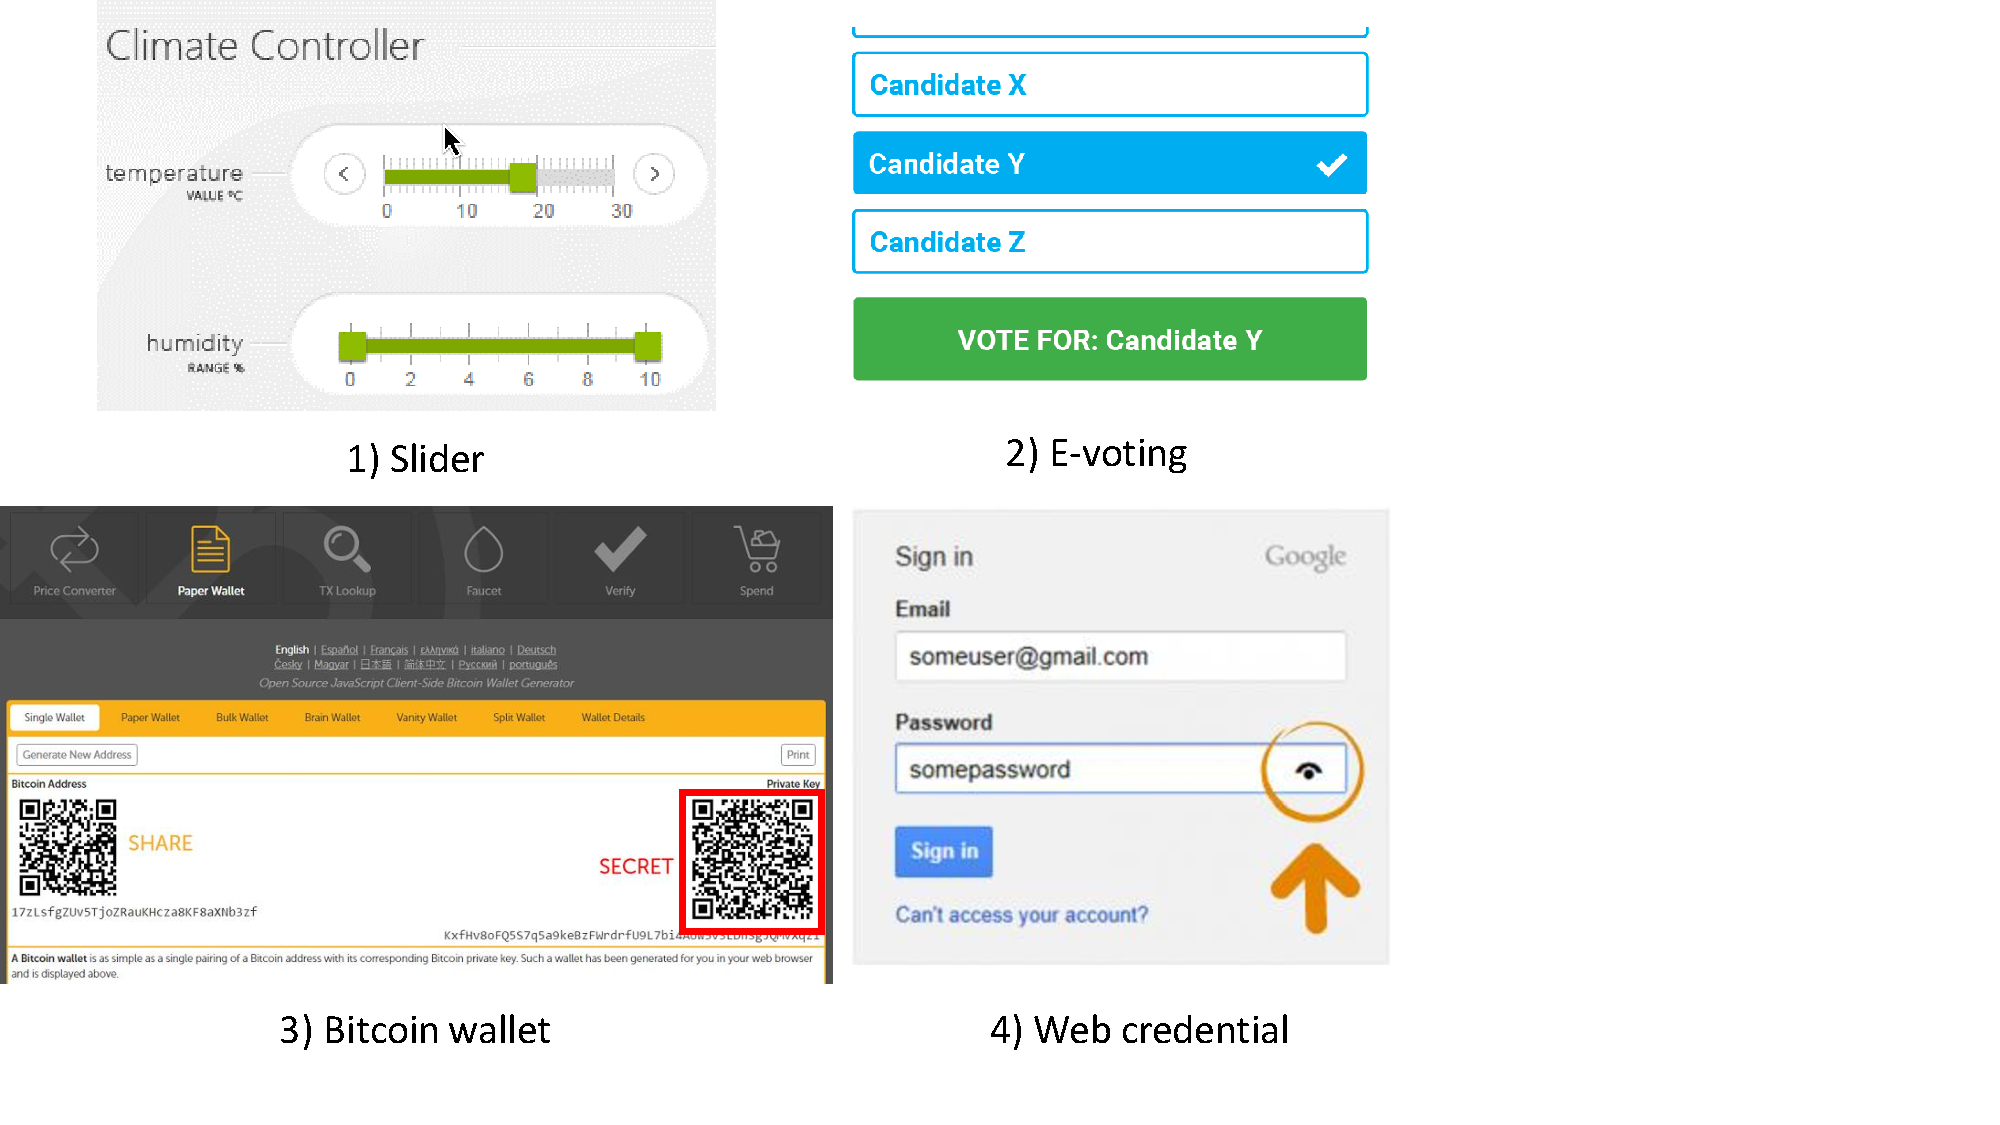
\includegraphics[trim={0 1cm 10cm 0}, clip, width=\linewidth]{motivation.pdf}
\caption{\textbf{Motivating examples.} 1) Pointer based UI elements that sets parameters to remote safety-critical device, 2) E-voting where the voting privacy and integrity is critical, 3) Financial transactions such as bitcoin wallet that shows sensitive information such as the user's private key and 4) web applications that provide an option for the user to reveal credentials.}
\spacesave
\label{fig:motivation}
\centering
\end{figure}


IO operation between the user and a remote server in the presence of an untrusted host is a long-standing problem. \emph{Trusted path} provides a secure channel between the user (HID) and the end-point where end-point is typically a trustworthy application running on the host. Trusted path ensures that input from the user is reached to the intended application, and all the outputs are generated by the legitimate application. Trusted path to the local host is a well-researched area where many solutions focus on using trusted software components such as a trusted hypervisor. In work done by Zhou et al.~\cite{zhou2012building}, the authors proposed a generic trusted path on $x86$ systems in pure hypervisor-based design. SGXIO~\cite{weiser2017sgxio} employed both the hypervisor and trusted execution environment (TEE) such as Intel SGX. Hypervisor requires too much TCB and often impractical in the real world scenario as most of the existing hypervisor offers very limited set of features.

However, when we consider an untrusted host, trusted path to the local host does not provide any advantage. In such an attacker model, it is crucial to ensure a trusted path from the user to a trusted remote server. Remote trusted path variant is non-trivial as typically all the IO operations are mediated by the operating system, device drivers, etc. Usage of an external trusted device is also another way to establish a trusted path. Transaction confirmation devices~\cite{filyanov2011uni,weigold2011secure} leverages on external device to confirm the input parameters. Such a device allows the user to review her input data on a separate trusted device that is physically separated from the untrusted host but suffers from poor usability and only limited to simple inputs. Bump in the Ether~\cite{McCPerRei2006} and IntegriKey~\cite{IntegriKey} uses an external embedded device to sign input parameters. However, such solutions ignore the view of the user context/view; hence, the attacker can execute UI manipulation attacks to trick the user into providing a wrong input.

Out of the numerous works, Fidelius~\cite{Fidelius} provides the most comprehensive solution to protect keyboard inputs from a compromised browser using \js that runs inside an SGX enclave. Fidelius uses overlays on display, specifically on the input text boxes to hide sensitive user input from the browser. But Fidelius suffers from both security and functional issues. Fidelius does not provide output integrity, such as the integrity of the layout of the UI and the labels. This allows the attacker to change instruction on the screen to influence user such as changing the unit of an input value to a safety-critical device. %Moreover, as the attacker model only consider the browser to be compromised~\footnote{\red{they consider a compromised host, but only trust sgx.}}, malicious enclave app, relay attack to the attacker's platform, etc., are out-of-scope of this paper. 
Also, Fidelius relies on an overlaid information bar that works as a \red{passive} security indicator. Several research works show that in real-world, \red{passive} security indicators do not provide adequate security, and suffer from user habituation. From the functional point of view, Fidelius only supports keyboard input and text box as input UI.
 
 
\myparagraph{Our contribution} The shortcomings of the previous works provide the groundwork of our paper which shows that without output integrity, input integrity is not achievable. \name is built upon the idea of delivering input integrity by first ensuring output integrity. \name also eliminates the need for security indicator to eliminate the risk of user habituation. \name leverages a trusted low-TCB auxiliary device that we call \device that works a generic IO hub between all user IO devices and the untrusted host. \device does not have any explicit network capability to communicate with the trusted remote server. Instead, the \device uses the host as an untrusted transport. \device ensures output integrity and confidentiality by sending an encoded UI to the host that only the \device can decode, and overlay on the display signal. The overlay is possible as the \device intercepts the display signal between the host and the monitor. The \device generated overlay ensures that the host can neither observe nor manipulate any output information; hence, it can not trick the user. The \device analyzes the intercepted HDMI frames to understand the correct user context, such as if the user moved her mouse over a specific UI element and click there. The \device also intercepts the mouse and keyboard signal and match them with the display signal that is received from the untrusted host. If both the input and output co-relates, the \device signs all the input and send them to the remote server. The signed input from the \device ensures input integrity and authenticity. 

In our design of \name, the \device acts as the \emph{root-of-trust} as the mere fact of connecting all the IO devices to the \device ensures the IO security. We can now summarize the contributions of \name as the following: 

\begin{mybullet}
  \item We describe the design of \name that provides integrity and confidentiality of user IO in an attacker-controlled environment, i.e., fully compromised host and the network. The design of \name leverages a small, low-TCB auxiliary device that acts as a \emph{root-of-trust} for the IO.
  \item \name provides mechanisms to protect the integrity of the mouse pointer activities alongside the keyboard, integrity and confidentiality of the UI, design to avoid user habituation, and provide users visual cues about the protected part of the screen. 
  \item We analyze the security of our solution in depth and prove that input integrity can only be achieved if output integrity is ensured. We also discuss potential side channel leakages that may undermine the confidentiality of IO. 
  \item We also provide an prototype implementation of \name that is practical and easy to use. Alongside of the prototype, we provide an evaluation of the prototype.
\end{mybullet}

\myparagraph{Organization of the paper} The organization of this paper is as the following. Section~\ref{sec:problemStatement} provides the detailed motivation, problem statement, state-of-the-art and the goals of this paper. Section~\ref{sec:approach} provides the system \& attacker model, challenges and a brief overview of our solution. We discussed the technical details of \name in Section~\ref{sec:systemDesign}. Section~\ref{sec:securityAnalysis} provides in-depth security analysis of \name. Section~\ref{sec:prototype} and~\ref{sec:eval} provide details of \name prototype implementation and corresponding evaluation. Finally, Section~\ref{sec:relatedWorks} and~\ref{sec:conclusion} provides the related research works and concludes the paper respectively.

%%%%%%%%%%%%%%%%%%%%%%%%%%%%%%%%%%%%%%
     %\myparagraph{State of the art} A trusted path provides roughly provide a set of four security properties to the communication channel between the user and the end system. Ensuring that the user performs intended actions to the remote server, typically, requires to assure that the user gets authentic output from the server. \emph{Output integrity} ensures that the information from the server reaches to the user in the intended form. For example, a user configuring a safety-critical device remotely bases her inputs in the current state of the system. As illustrated in the Figure~\ref{fig:motivation}, a compromised host could trick the user into performing unintended actions by providing incorrect feedback about the actual status. \emph{Output confidentiality} enables applications that require that the trusted paths offer a mechanism for the remote server to show secret information to the user. Figure~\ref{fig:motivation} illustrates such cases when a web server delivers a private key of a crypto-wallet to the user which should be kept hidden to the untrusted host.

%Once that output security is achieved, the trusted paths should guarantee that the remote servers accept only inputs generated by the honest user - \emph{Input integrity}. This feature is critical for the integrity of user actions in case of a compromised host. As shown in Figure~\ref{fig:motivation}, the user submits her inputs, and the remote server assures that a malicious host has not altered the user's original inputs. \emph{Input confidentiality} provides stricter security guarantees. Other applications (e.g., e-voting) require a higher level of security, the inputs should be sent to the server as generated by the user---input integrity---and preferably the host should not have access to inputs. Note that, to provide input security, trusted paths should guarantee at first output security.


%Trusted path is in focus in several recent research works. Several ways could be employed to realize the trusted path. For example, Filyanov et. al~\cite{filyanov2011uni} proposed transaction confirmation device that requires the user to use a separate device to confirm the input parameters. This allows the user to review her input data on a separate trusted device that is physically separated from the untrusted host. Trusted execution environments (TEE) such as Intel SGX, ARM TrustZone, TPM, Intel TXT, etc. provide isolated code execution, and can be used to achieve trusted path. Previous research works such as Intel SGX and trusted hypervisor-based SGXIO~\cite{weiser2017sgxio}, Intel SGX based ProximiTEE~\cite{dhar2018proximitee}, TPM and TXT based trusted path~\cite{filyanov2011uni}, and ARM TrustZone based trusted path~\cite{sun2015trustotp} are the example of trusted path construction based on TEEs. All of these solutions require specialized platforms with processors that support such infrastructure. VButton~\cite{li2018vbutton} uses ARM TrustZone to overlay buttons on the mobile devices that confirm if the user taps on a specific button. Processor-TEE such as Intel SGX primarily provides execution privacy and code integrity. In most of the cases, IO is still mediated by the OS. InContext~\cite{huang2012clickjacking} presents different clickjacking attacks variants and their solution by ensuring context (both temporal and visual) and pointer integrity in the trusted browser setting. Trusted hypervisors and secure micro-kernels are also choices for contrasting Trusted path. Sel4~\cite{klein2009sel4} is a functional hypervisor that is formally verified and has a kernel size of only $8400$ lines of code. In work done by Zhou et al.~\cite{zhou2012building}, the authors proposed a generic trusted path on $x86$ systems in pure hypervisor-based design. Examples of other hypervisor-based works can be found in systems such as Overshadow~\cite{Overshadow}, Virtual ghost~\cite{criswell2014virtual}, Inktag~\cite{hofmann2013inktag}, TrustVisor~\cite{mccune2010trustvisor}, Splitting interfaces~\cite{ta2006splitting}, $SP^3$~\cite{yang2008using}, etc.

%In spite of numerous existing research works on trusted path, none of the existing system provides an end-to-end secure trusted path that works on generic input devices, handles complex UI and user interactions, and introduces minimal or no changes to the existing systems and user's behaviour. This leads to the realization of our proposed solution, \name.


 